\documentclass{article}
\usepackage[utf8]{inputenc}
\usepackage[letterpaper, portrait, margin=0.2in]{geometry}
\usepackage{multicol}
\usepackage{amsmath}
\usepackage{amssymb}
\usepackage{enumerate}
\usepackage{esint}
\setlength\parindent{0pt}
\usepackage{enumerate}
\usepackage{graphicx}
\graphicspath{ {../images/} }
\usepackage{fancyhdr}
\usepackage{tcolorbox}
\usepackage[fontsize=7pt]{fontsize}
\usepackage[none]{hyphenat}
\usepackage[document]{ragged2e}
\newcommand{\sheader}[1]{\underline{#1:}}
\usepackage{physics}

\newcommand{\sepvec}{\vec{r_\textrm{sep}}}
\newcommand{\sephat}{\hat{r}_{\textrm{sep}}}
\newcommand{\kfrac}{\frac{1}{4\pi\epsilon_0}}
\newcommand{\ds}{\displaystyle}


\newcommand{\header}[1]{\begin{large}\noindent #1\end{large}\\\rule{\textwidth}{0.5pt}}
\newcommand{\gap}{\medskip\\}
\newcommand{\centertext}[1]{\begin{center}#1\end{center}}
\newcommand{\bfrac}[2]{\left(\frac{#1}{#2}\right)}
\newcommand{\formula}[2]{\begin{center} \begin{tcolorbox}[title = #1, boxrule=2pt,arc=3.4pt,boxsep=0mm] $$#2$$\end{tcolorbox}\end{center}}
\newcommand{\doubleformula}[3]{\begin{center} \begin{tcolorbox}[title = #1, boxrule=2pt,arc=3.4pt,boxsep=0mm] $$#2$$\\$$#3$$\end{tcolorbox}\end{center}}
\newcommand{\formulax}[2]{\underline{#1}\smallskip\centering $#2$ \raggedleft}
\newcommand{\tripleformula}[4]{\begin{center} \begin{tcolorbox}[title = #1, boxrule=2pt,arc=3.4pt,boxsep=0mm] \begin{align*} #2 \\ #3 \\ #4\end{align*}
    \end{tcolorbox}\end{center}}

\newcommand{\formbox}[2]{\begin{center} \begin{tcolorbox}[colback=white, title = #1, boxrule=2pt,arc=3.4pt,boxsep=0mm] #2\end{tcolorbox}\end{center}}


\newcommand{\where}{\hspace{0.3cm} \textrm{where} \hspace{0.3cm}}
\usepackage{array}
\begin{document}


\begin{multicols*}{2}
    \formbox{Electrostatics Basics}{
        {\renewcommand{\arraystretch}{1.75}%
        \begin{tabular}{ m{12em} m{25em}  }
            Line Charge: & $\displaystyle \vec{E}(\vec{r}) = \frac{1}{4 \pi \epsilon_0}\int{\frac{\lambda(\vec{r'})}{||\sepvec||^2}\sephat \, dl'}$\\
            Surface Charge: & $\displaystyle \vec{E}(\vec{r}) = \frac{1}{4\pi\epsilon_0}\int{\frac{\sigma(\vec{r'})}{||\sepvec||^2}\sephat \, da'}$\\
            Volume Charge: & $\displaystyle \vec{E}(\vec{r}) = \frac{1}{4\pi\epsilon_0}\int{\frac{\rho(\vec{r'})}{||\sepvec||^2}\sephat \, d\tau'}$\\
            Potential Difference: & $\displaystyle V(\vec{b}) - V(\vec{a}) = - \int_{\vec{a}}^{\vec{b}}{\vec{E} \cdot d\vec{l}}$\\
            Potential of a Volume Charge: & $\displaystyle V(\vec{r}) = \kfrac \int{\frac{\rho(\vec{r'})}{||\sepvec||}d\tau'}
            $\\
            Potential of a Collection of Point Charges: & $\displaystyle V(\vec{r}) = \kfrac \sum_{i = 0}^n\frac{q_i}{||\sepvec||}$\\
            Work to Move a Charge: & $\displaystyle {W = \int_{\textbf{a}}^{\textbf{b}} \vec{F} \cdot d\vec{l} = -Q\int_{\textbf{a}}^{\textbf{b}}{\vec{E} \cdot d\vec{l}}}$\\
            Work to Move a Charge (Potential): & $\displaystyle {W= Q[V(\vec{b}) - V(\vec{a})]}$\\
            Energy of a Collection of Point Charges: & $\displaystyle W = \frac{1}{2}\sum_{i = 1}^n{q_i V(\vec{r_i})}$\\
            Energy of a Continuous Charge Distribution: & $\displaystyle W = \frac{\epsilon_0}{2}\int\limits_{\textrm{univ}}E^2 d\tau = \frac{1}{2}\iiint \rho V d\tau$\\
            Field at a Charged Surface: & $\displaystyle \vec{E}_\textrm{surf} = \frac{1}{2} \left( \vec{E}_\textrm{above} + \vec{E}_\textrm{below}\right)$\\
            Parallel Plate Voltage: & $\displaystyle V = \frac{Q}{A\epsilon_0}d$\\
            Capacitance: & $\displaystyle C \equiv \frac{Q}{V}$\\
            Energy of a Capacitor: & $\displaystyle W = \int_0^Q{\bfrac{q}{C}dq} = \frac{1}{2}\frac{Q^2}{C} = \frac{1}{2} CV^2$\\

        \end{tabular}}
    }
    \formbox{Electrostatic Multipoles}{
        {\renewcommand{\arraystretch}{2}%
        \begin{tabular}{ m{8em} m{30em}  }
            Generalized Multipole Expansion: & $\displaystyle V(r) = \frac{1}{4\pi \epsilon_0}\sum_{n = 0}^\infty \frac{1}{r^{n + 1}} \int_{V} ||\vec{r'}||^n P_n(\cos \alpha)\rho(\vec{r'})d\tau'$\\
        \end{tabular}}
        \begin{tabular}{ m{15em} m{20em}  }
            Monopole Voltage: & $\displaystyle V(r) = \kfrac\frac{Q}{r}$\\
            Dipole Voltage: & $\displaystyle V(r) = \kfrac \frac{\vec{p}\cdot \hat{r}}{r^2}$\\
            Dipole Moment (Continuous): & $\displaystyle \vec{p} \equiv \int_V \vec{r'}\rho(\vec{r'})d\tau'$\\
            Dipole Moment (Discrete): & $\displaystyle \vec{p} = \sum_{i = 1}^n q_i \vec{r'}_i$\\
            Dipole Moment (Change of Origin): & $\vec{p'} = \vec{p} - Q\vec{a}$\\
            Torque of a Dipole: & $\displaystyle \vec{N} = \vec{p} \times \vec{E}$\\
            Energy of a Dipole: & $\displaystyle U = -\vec{p} \cdot \vec{E}$\\
            Force on a Dipole: & $\displaystyle \vec{F} = (\vec{p} \cdot \nabla)\vec{E}$\\
            Field of a Dipole: & $\displaystyle \vec{E} = \kfrac\frac{p}{r^2}\left(2 \cos \theta \hat{r} + \sin \theta \hat{\theta}\right)$
        \end{tabular}
    }
    \formbox{Electrostatics in Matter}{
        {\renewcommand{\arraystretch}{1.75}%
        \begin{tabular}{ m{12em} m{25em}  }
            Electric Displacement: & $\displaystyle \vec{D} \equiv \epsilon_0 \vec{E} + \vec{P}$\\
            Bound Surface Charge: & $\displaystyle \sigma_\textrm{bound} = \vec{P} \cdot \hat{n}$\\
            Bound Volume Charge: & $\displaystyle \rho_\textrm{bound} \equiv -\nabla \cdot \vec{P}$\\
            Linear Dielectrics -- Polarization: & $\displaystyle \vec{P} = \epsilon_0 \chi_e \vec{E}$\\
            Linear Dielectrics -- E-Field: & $\displaystyle \vec{D} = \epsilon \vec{E}$\\
            Electric Permittivity: & $\displaystyle \epsilon = \epsilon_0 (1 + \chi_e) = \epsilon_0 \epsilon_r$\\
            Gauss's Law for $\vec{D}$ (Derivative): & $\displaystyle \nabla \cdot \vec{D} = \rho_f$\\
            Gauss's Law for $\vec{D}$ (Integral): & $\displaystyle \oint\vec{D} \cdot d\vec{A} = Q_{f_\textrm{encl}}$\\
            Force on a Dielectric: & $F = -\nabla U$\\
            Energy of a Dielectric: & $W = \frac{1}{2}\int \vec{D} \cdot \vec{E} d\tau$
        \end{tabular}}
    }
    \formbox{Names of Stuff}{
        $\epsilon_0$: Permittivity of Free Space\\
        $\epsilon_r$: Dielectric Constant or Relative Permittivity\\
        $\epsilon$: Permittivity of a Material
    }
    PHYS 301 Formula Sheet. Critchlow/Wilson/Predinchuk 2022.
    \formbox{Techniques for Solving Problems}{
        {\renewcommand{\arraystretch}{1.75}%
        \begin{tabular}{ l }
            Cylindrical Laplacian Solution:\\
            $\displaystyle V(s, \phi) = A \ln s +
            B + \sum_{n = 1}^\infty \left(A_n s^n + \frac{B_n}{s^n}\right)
            \left(C_n \cos (\phi n) + D_n \sin(\phi n)\right)$\\
        \end{tabular}
        \begin{tabular}{ m{12em} m{20em}  }
            Solution for Spherical Laplacians: & $\displaystyle V(r, \theta) = \sum_{l = 0}^\infty{\left(A_l r^l + \frac{B_l}{r^{l + 1}}\right)P_l(\cos \theta)}$\\
            Method of Images General Principle: & $\displaystyle \sum \frac{q_i}{||\sepvec_i||} = 0$\\
            Method of Images for Two Points: & $\displaystyle -\frac{q_1}{q_2} = \frac{||\sepvec_1||}{||\sepvec_2||}$\\
            Image Charge Surface Charge: & $\displaystyle \sigma = - \epsilon_0 \frac{\partial V}{\partial n}$\\
            Binomial Expansion: & $(1+x)^n = 1 + n x + \frac{n(n-1)}{2!}x^2 + \frac{n(n-1)(n-2)}{3!}x^3 + \cdots + n x^{n-1} + x^n.$\\
            Taylor Expansion: & $\displaystyle f(x) \approx \sum_{n=0}^\infty \frac{f^{(n)}(0)}{n!}$\\
            Because I can't remember: & $\displaystyle f(x) \approx f(0) + f'(0) \cdot x + f''(0) \cdot \frac{x^2}{2} + \cdots$\\
            Legendre Polynomials: &
            {\renewcommand{\arraystretch}{1}%       
            \begin{tabular}{l}          
            $P_0(\cos \theta) = 1$\\
            $P_1(\cos \theta) = \cos\theta$ \\
            $P_2(\cos \theta) = \frac{3}{2} \cos^2 \theta - \frac{1}{2}$\\
            $P_3(\cos \theta) = \frac{5}{2} \cos^3 \theta - \frac{3}{2} \cos \theta$
            \end{tabular}}
        \end{tabular}
        }
    }
    \formbox{Magnetostatics}{
        {\renewcommand{\arraystretch}{2}%
        \begin{tabular}[t]{ m{13em} m{25em}  }
            Lorentz Force Law: & $\displaystyle \vec{F}_\textrm{mag} = Q(\vec{v} \times \vec{B})$\\
            Surface Current Density: & 
            {\renewcommand{\arraystretch}{1}%       
            \begin{tabular}[t]{l}          
                $\displaystyle \vec{K} \equiv \frac{d\vec{I}}{dl_\perp}$
                \\
                $\displaystyle \vec{K} = \sigma \vec{v}$
            \end{tabular}}\\
            Volume Current Density: &
            {\renewcommand{\arraystretch}{1}%       
            \begin{tabular}[t]{l}          
                $\displaystyle J \equiv \frac{d\vec{I}}{da_\perp}$
                \\
                $\displaystyle \vec{J} = \rho\vec{v}$
            \end{tabular}}\\
            Magnetic Force (General): & $\displaystyle \vec{F}_\textrm{mag} = \int I(d\vec{l} \times \vec{B}) = I \int (d\vec{l} \times \vec{B})$\\
            Magnetic Force (Surface): & $\displaystyle \vec{F}_\textrm{mag} = \int (\vec{K} \times \vec{B})da$\\
            Magnetic Force (Volume): & $\displaystyle \vec{F}_\textrm{mag} = \int (\vec{J} \times \vec{B}) d\tau$\\
            Biot-Savart Law: & 
            {\renewcommand{\arraystretch}{1}%       
            \begin{tabular}[t]{l}          
                $\displaystyle \vec{B}(\vec{r}) = \frac{\mu_0}{4\pi} \int \frac{\vec{I} \times \hat{r}_\textrm{sep}}{||\sepvec||^2} dl'$
                \\$\displaystyle \vec{B}(\vec{r}) = 
                \frac{\mu_0}{4\pi}I \int \frac{d\vec{l}'\times \hat{r}_\textrm{sep}}{||\sepvec||^2}$
            \end{tabular}}\\
            Biot-Savart -- Surface: &
            $\ds \vec{B}(\vec{r}) =  \frac{\mu_0}{4\pi}\int \frac{\vec{K}(\vec{r'}) \times \sephat}{||\sepvec||^2}da'$\\
            Biot-Savart -- Volume: &
            $\ds \vec{B}(\vec{r}) = \frac{\mu_0}{4\pi}\int \frac{\vec{J}(\vec{r'}) \times \sephat}{||\sepvec||^2}d\tau'$\\
            Ampere's Law: &
            {\renewcommand{\arraystretch}{1}%       
            \begin{tabular}[t]{l}          
                $\displaystyle  \vec{\nabla} \times \vec{B} = \mu_0\vec{J}$
                \\
                $\displaystyle \oint \vec{B} \cdot d\vec{l} = \mu_0 I_\textrm{encl}$
            \end{tabular}}\\
            Magnetic Vector Potential: &
            {\renewcommand{\arraystretch}{1}%       
            \begin{tabular}[t]{l}          
                $\displaystyle  \vec{B} = \vec{\nabla} \times \vec{A}$
                \\
                $\displaystyle \vec{\nabla} \cdot \vec{A} = 0$
                \\
                $\displaystyle  \nabla^2 \vec{A} = -\mu_0 \vec{J}$
            \end{tabular}}\\
            Vector Potential -- Line: & $\displaystyle \vec{A} = \frac{\mu_0}{4\pi} \int \frac{\vec{I}}{||\sepvec||}dl' = \frac{\mu_0 I}{4\pi} \int \frac{1}{||\sepvec||}d \vec{l'}$\\
            Vector Potential -- Surface: & $\displaystyle \vec{A} = \frac{\mu_0}{4\pi}\int \frac{\vec{K}}{||\sepvec||}da'$\\
            Vector Potential -- Volume: & $\displaystyle \vec{A} = \frac{\mu_0}{4\pi} \int \frac{\vec{J}(\vec{r'})}{||\sepvec||}d\tau'$\\
            Magnetic Dipole Moment: & $ \displaystyle  \vec{m} \equiv I \int d\vec{a} = I \vec{a}$\\
            Magnetic Dipole Potential Expansion: & $\displaystyle \vec{A}_\textrm{dip}(\vec{r}) = \frac{\mu_0}{4\pi} \frac{\vec{m} \times \hat{r}}{r^2}$\\
            Magnetic Torque: & $\displaystyle \vec{N} = \vec{m} \times \vec{B}$\\
            Energy of a Dipole: & $\ds U = -\vec{m} \cdot \vec{B}$\\
            Force on a Magnetic Dipole: & $\displaystyle \vec{F} = \nabla(\vec{m} \cdot \vec{B})$\\
            Force Between Two Current-Carrying Wires: & $\displaystyle \frac{F}{l} = \frac{\mu_0 I_1 I_2}{2\pi r}$\\
            Linear Current: & $\ds \vec{I} = \int \vec{K} \cdot d \vec{l} = \iint \vec{J}\cdot d\vec{a}$
        \end{tabular}}
    }
    \formbox{Maxwell's Equations}{
        {\renewcommand{\arraystretch}{1.75}%
        \begin{tabular}{ m{7em} m{10em} m{12em}  }
            Gauss's Law: & $\displaystyle \vec{\nabla} \cdot \vec{E} = \frac{1}{\epsilon_0}\rho$ & $\displaystyle\oiint \vec{E}\cdot\vec{da} = \frac{Q_{enc}}{\epsilon_0}$\\
            No monopoles: & $\displaystyle \vec{\nabla} \cdot \vec{B} = 0$ & $\displaystyle \oiint\vec{B}\cdot d\vec{a}=0$\\
            Faraday's Law: & $\displaystyle \vec{\nabla} \times \vec{E} = -\frac{\partial \vec{B}}{\partial t}$ & $\displaystyle\oint\vec{E}\cdot\vec{dl} = \frac{-\partial \Phi_{B}}{\partial t}$\\
            \small{Ampere's Law with Maxwell's Correction:} & \small{$\displaystyle \vec{\nabla} \times \vec{B} = \mu_0 \vec{J} + \mu_0\ \epsilon_0 \frac{\partial \vec{E}}{\partial t}$} & \small{$\displaystyle \oint\vec{B}\cdot d\vec{l}=\mu_0I_{enc}+\mu_0\epsilon_0\frac{\partial \Phi_E}{\partial t}$}\\
        \end{tabular}}
    }
    \formbox{Magnetostatics in Matter}{
        {\renewcommand{\arraystretch}{1.75}%
        \begin{tabular}{ m{12em} m{20em}  }
            Paramagnets: & magnetization is \textbf{parallel} to $\vec{B}$\\
            Diamagnets: & magnetization is \textbf{opposite} to $\vec{B}$\\
            Ferromagnets: & magnetization holds outside the presence of an 
            external magnetic field.\\
            Magnetization: & $\displaystyle \vec{M} \equiv$ magnetic dipole per unit volume\\
            Bound Volume Current: & $\displaystyle  \vec{J}_\textrm{bound} = \vec{\nabla} \times \vec{M}$\\
            Bound Surface Current: & $\displaystyle \vec{K}_\textrm{bound} = \vec{M} \times \hat{n}$\\
            Free Current: & $\displaystyle \vec{J} = \vec{J}_b + \vec{J}_f$\\
            Auxillary Field: & $\displaystyle \vec{H} \equiv \frac{1}{\mu_0}\vec{B} - \vec{M}$\\
            Ampere's Law for Auxillary Fields: &
            {\renewcommand{\arraystretch}{1}%       
            \begin{tabular}[t]{l}          
                $\displaystyle \vec{\nabla} \times \vec{H} = \vec{J}_f$
                \\
                $\displaystyle \oint \vec{H} \cdot d\vec{l} = I_{f_\textrm{encl}}$
            \end{tabular}}\\
            Linear Magnetics: & $\displaystyle \vec{M} = \chi_m\vec{H}$\\
            Permeability: & $\displaystyle \mu \equiv \mu_0(1 + \chi_m)$\\
            Relative Permeability: & $\ds \mu_r =  1 + \chi_m$\\
            Linear Magnetics with E and H Fields: & $\displaystyle \vec{B} = \mu \vec{H}$.\\
            Dipole Field: & $\ds \vec{B} = \frac{\mu_0 m}{4\pi r^3}(2\cos(\theta)\hat{r} + \sin(\theta)\hat{\theta})$, for $\vec{m} = m\hat{z}$\\
            Field Inside a Uniformly Magnetized Sphere: &
            $\vec{B} = \frac{2}{3}\mu_0 \Vec{M}$\\
            Really?: & $\vec{J}_b = \chi_m \vec{J}_f$\\
            Force on a dipole moment: & $\Vec{F} = \nabla (\vec{m} \cdot \Vec{B})$
        \end{tabular}}
    }
    \formbox{Electrodynamics}{
        {\renewcommand{\arraystretch}{1.75}%
        \begin{tabular}{ m{12em} m{25em}  }
            Ohm's Law: & $\displaystyle V = IR$\\
            Power in a Circuit: & $\displaystyle P = VI = I^2R = \frac{V^2}{R}$\\
            Electromotive Force: &
            \begin{tabular}[t]{l}          
                $\displaystyle \mathcal{E} = \frac{F_\textrm{mag, tot}}{Q} = \int (\vec{v} \times \vec{B})\cdot d \vec{l}$\\
                $\displaystyle  \mathcal{E} = \oint \vec{f} \cdot d \vec{I}$
                \\
                $\displaystyle \mathcal{E} = - \frac{d\Phi}{dt}$
            \end{tabular}\\
            Faraday's Law: & $\displaystyle \vec{\nabla} \times \vec{E} = - \frac{\partial \vec{B}}{\partial t}$\\
            Inductance: &
            \begin{tabular}[t]{l}          
                $\displaystyle  \Phi = LI$
                \\
                $\displaystyle \mathcal{E} = -L \frac{dI}{dt}$
            \end{tabular}\\
            Work of a Magnetic Field: &
            \begin{tabular}[t]{l}          
                $\displaystyle \frac{1}{2} LI^2$
                \\
                $\displaystyle W = \frac{1}{2\mu_0}\int_\textrm{all space}B^2 d\tau$
            \end{tabular}\\
            Displacement Current: & $\vec{J}_d \equiv \epsilon_0\frac{\partial \vec{E}}{\partial t}$\\
            Faraday's Law in Integral Form: &
            $\ds \oint \vec{E} \cdot d \vec{l} = - \frac{d \Phi}{dt}$
        \end{tabular}}
    }
    \formbox{Maxwell's Equations in Matter}{
        {\renewcommand{\arraystretch}{1.75}%
        \begin{tabular}{ m{12em} m{25em}  }
            Gauss's Law: & $\displaystyle \vec{\nabla} \cdot \vec{D} = \rho_f$\\
            (unnamed) & $\displaystyle \vec{\nabla} \cdot \vec{B} = 0$\\
            Faraday's Law: & $\displaystyle \vec{\nabla} \times \vec{E} = - \frac{\partial \vec{B}}{\partial t}$\\
            Ampere's Law with Maxwell's Correction: & $\displaystyle \vec{\nabla} \times \vec{H} = \vec{J}_f + \frac{\partial \vec{D}}{\partial t}$\\
        \end{tabular}}
    }
    \formbox{Triangles}{
        \begin{center}
            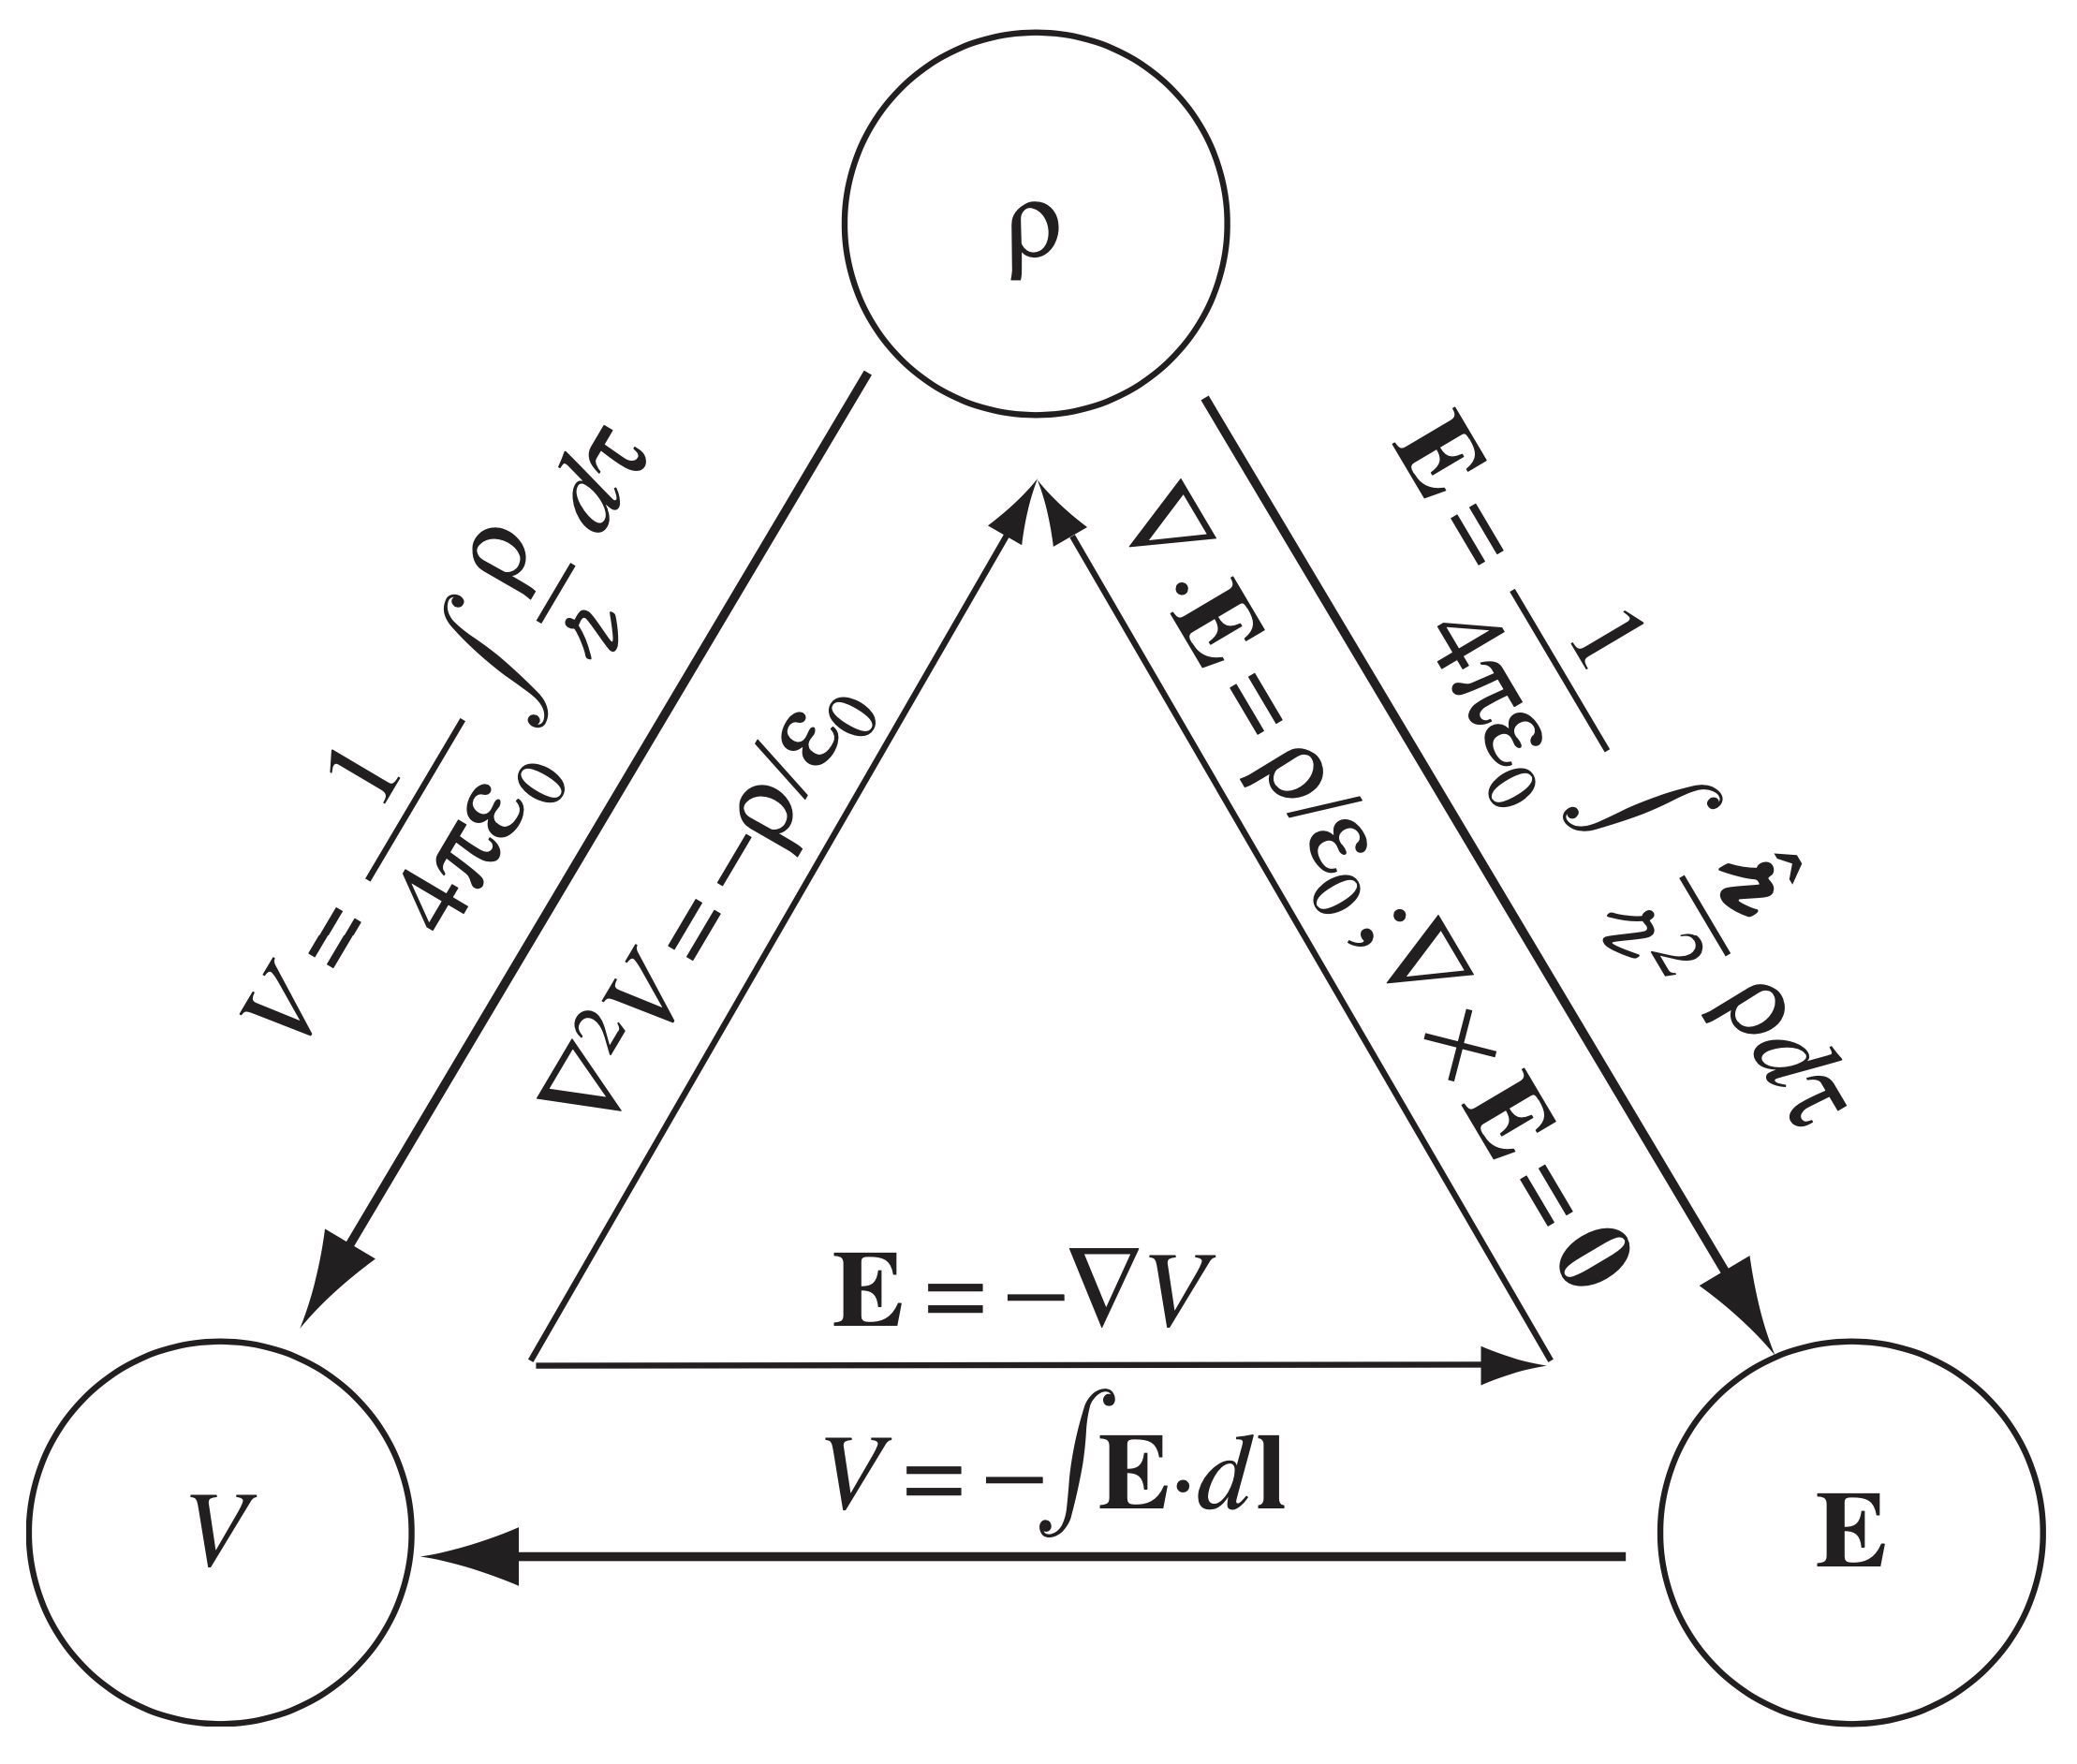
\includegraphics[height=3.4cm]{em-triangle.png}
            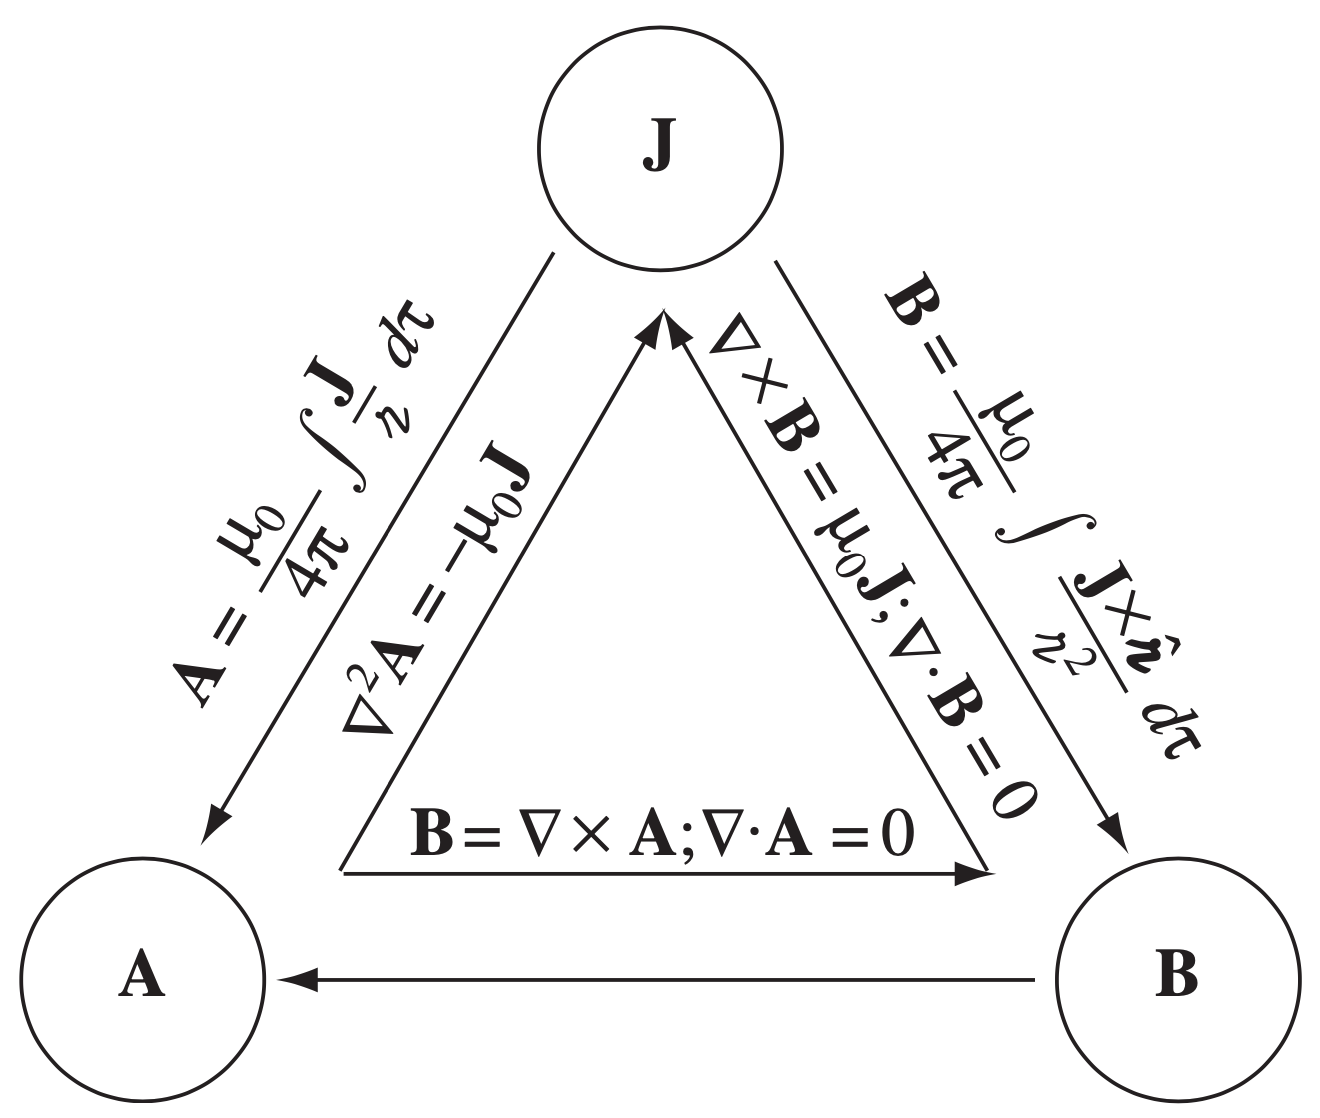
\includegraphics[height=3.8cm]{magnetic-triangle.png}
        \end{center}
    }

    \formbox{Boundary Conditions in Electrostatics}{
        {\renewcommand{\arraystretch}{1.75}%
        \begin{tabular}{ l l }
            $\vec{D}_{\text{above}}^{\perp} - \vec{D}_{\text{below}}^{\perp}  = \sigma_f$&
            $V_\text{above} = V_\text{below}$
            \\
            $\vec{E}_{\text{above}}^{\perp} - \vec{E}_{\text{below}}^{\perp}  = \sigma_{\text{tot}}/\epsilon_0$&
            $\vec{E}_{\text{above}}^{\parallel} - \vec{E}_{\text{below}}^{\parallel}  = \vec{0}$\\
            $\vec{D}_{\text{above}}^{\parallel} - \vec{D}_{\text{below}}^{\parallel} = \vec{P}_{\text{above}}^{\parallel} - \vec{P}_{\text{below}}^{\parallel}$&
            $\epsilon_\text{above}\vec{E}_\text{above}^\perp - \epsilon_\text{below}\vec{E}_\text{below}^\perp = \sigma_f$\\
            $\ds \epsilon_\text{above}\pdv{V_\text{above}}{n} - \epsilon_\text{below}\pdv{V_\text{below}}{n} = -\sigma_f$
        \end{tabular}}
    }
    \formbox{Boundary Conditions in Magnetostatics}{
        {\renewcommand{\arraystretch}{1.75}%
        \begin{tabular}{ l l }
            $\vec{B}_\text{above}^\parallel - \vec{B}_\text{below}^\parallel = \mu_0\vec{K}$ &
            $\vec{B}_\text{above} - \vec{B}_\text{below} = \mu_0(\vec{K}\cross\vu{n})$\\
            $\vec{A}_\text{above} = \vec{A}_\text{below}$&
            $\ds \pdv{A_\text{above}}{n} - \pdv{A_\text{below}}{n} = -\mu_0\vec{K}$\\
            $\vec{H}_\text{above}^\perp - \vec{H}_\text{below}^\perp = - (\vec{M}_\text{above}^\perp - \vec{M}_\text{below}^\perp) $&
            $\vec{H}_\text{above}^\parallel - \vec{H}_\text{below}^\parallel = \vec{K}_f \cross \vu{n}$
        \end{tabular}}
    }
    \formbox{More Boundary Conditions}{
        \begin{center}
            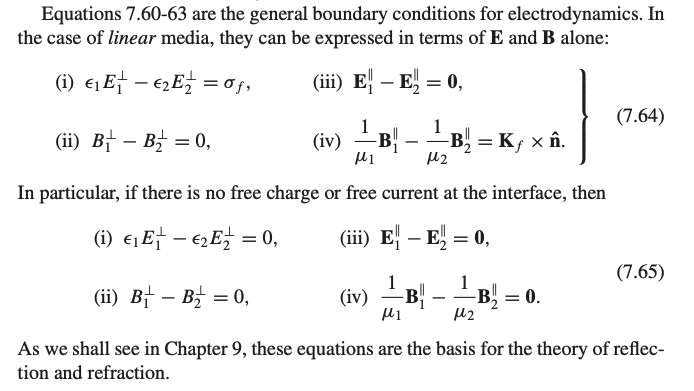
\includegraphics[width=8cm]{boundary-conditions.png}
        \end{center}
    }
    \formbox{Common Fields}{
        {\renewcommand{\arraystretch}{2}%
        \begin{tabular}{ m{12em} m{25em}  }
            E and V for inf line: & $\displaystyle E(s) = \frac{\lambda}{2\pi\epsilon_0 s}, V(s) = \frac{\lambda}{2\pi\epsilon_0}\ln{|\frac{s_0}{s}|}$\\
            E and V for inf plane: & $E = \frac{|\sigma|}{2\epsilon_0}, V = \mp\frac{\sigma z}{2\epsilon_0} $\\
            E and V at $(0,0,z)$ of ring: & $E(z) = \frac{\lambda z R}{2\epsilon_0(R^2+z^2)^{\frac{3}{2}}}, V(z) = \frac{\lambda \cdot R}{2\epsilon_0\sqrt{R^2+z^2}}$\\
            E and V at $(0,0,z)$ of disk: & 
            \begin{tabular}[t]{l}          
                $E(z) = \frac{\sigma}{2\epsilon_0}[1 - \frac{z}{\sqrt{z^2+R^2}}]$
                \\
                $V(z) = \frac{\sigma}{2\epsilon_0}[\sqrt{R^2+z^2} - |z|]$
            \end{tabular}\\
            E and V for uniform hollow sphere: & 
            \begin{tabular}[t]{l}          
                $E(r) = \frac{\sigma R^2}{\epsilon_0 r^2}u(r-R)$
                \\
                $V(r) = \frac{\sigma R}{\epsilon_0 }u(R-r) + \frac{\sigma R^2}{\epsilon_0 r}u(r-R)$
            \end{tabular}\\
        
            Magnetic Wire: & $\displaystyle \frac{\mu_0}{4\pi}\frac{I}{r}(\sin (\theta_1) - \sin (\theta_2))$\\
            Magnetic Sheet: & $B = \frac{\mu_0K}{2}$\\
            Magnetic Field of an Arc Along z: & $\displaystyle \frac{\mu_0 I R^2 \theta}{4\pi (z^2+R^2)^{3/2}}$\\
            % Magnetic Field of an Infinite Wire: & $\displaystyle \frac{\mu_0 I}{2\pi R}$\\
            Magnetic Field of a Solenoid: & $\ds \mu_0 n I$\\
            B-field in thin magnetized cylinder: & $B = \mu_0M$\\
            B-field in magnetized sphere: & $B = \frac{2}{3}\mu_0M = \frac{2}{3}\mu_0\sigma R \omega \text{ for spinning sphere}$
            
        \end{tabular}}
    }
\end{multicols*}


\end{document}